\documentclass[11pt,a4paper]{article}
\usepackage[utf8]{inputenc}
\usepackage[english]{babel}
\usepackage{geometry}
\usepackage{amsmath,amsfonts,amssymb}
\usepackage{graphicx}
\usepackage{float}
\usepackage{booktabs}
\usepackage{longtable}
\usepackage{array}
\usepackage{multirow}
\usepackage{hyperref}
\usepackage{xcolor}
\usepackage{listings}
\usepackage{caption}
\usepackage{subcaption}
\usepackage{titlesec}

% Formattazione di sezioni e sottosezioni senza colore
\titleformat{\section}
  {\Large\bfseries}
  {\thesection}{1em}{}

\titleformat{\subsection}
  {\large\bfseries}
  {\thesubsection}{1em}{}

\definecolor{success}{RGB}{46, 160, 67}
\definecolor{warning}{RGB}{255, 193, 7}
\definecolor{danger}{RGB}{220, 53, 69}

\begin{document}
\begin{titlepage}
    \centering
    \vspace*{2cm}
    
    {\Huge\bfseries Performance Analysis of Heuristics in Answer Set Programming}
    
    \vspace{1.5cm}
    
    {\Large A Comprehensive Study on Optimization Techniques for ASP-based Operational Room Scheduling}
    
    \vspace{10.5cm}

    {\large \today}
    
    \vfill
\end{titlepage}

\newpage

\section{Executive Summary}

This research project investigates the application of heuristics within Answer Set Programming (ASP) encodings for the Operational Room Scheduling problem, with the objective of accelerating the discovery of optimal solutions. The study focuses on two critical performance metrics: the time required to identify the first feasible solution and the time necessary to achieve global optimality.

Our empirical analysis, conducted across a dozen specialized heuristics, demonstrates that while heuristics may not substantially improve the time to discover the first answer set or reach the optimal solution, they provide significant enhancements in proving global optimality. Specifically, we observed speedup factors of up to 6.65 times faster than baseline implementations when confirming that a solution represents the global minimum.

The comprehensive evaluation encompasses 40 distinct problem instances across varying complexity levels, providing robust empirical evidence for the effectiveness of targeted heuristic approaches in ASP-based optimization. Additionally, we modified the structure of the choice rule and the primary constraint of the original encoding to reduce the number of generated answer sets, thereby improving solution search efficiency without compromising solution quality.

\section{Research Methodology}

\subsection{Experimental Design}

The research methodology follows a systematic four-phase approach designed to identify, evaluate, and optimize heuristic combinations for ASP problem solving:

\textbf{Phase 1: Heuristic Collection} - Potentially effective heuristics for the operational room scheduling domain were collected and stored in the file \texttt{0\_heuristics\_to\_try.lp}. This initial collection was based on domain knowledge and established ASP optimization principles.

\textbf{Phase 2: Individual Heuristic Evaluation} - The script \texttt{1\_brute\_force\_heuristic\_extractor.py} was executed to systematically extract and evaluate each heuristic from the collection file. Each heuristic was tested individually on the input instance specified in \texttt{settings.json}. Heuristics demonstrating improvements in either first solution discovery time or global optimality achievement time were classified as promising and saved to \texttt{2\_promising\_ones.lp}.

\textbf{Phase 3: Combinatorial Analysis} - The script \texttt{3\_combine\_heuristics.py} was employed to evaluate all possible combinations of the promising heuristics identified in Phase 2. This comprehensive combinatorial analysis was performed on the same input instance, with results systematically recorded in \texttt{timings\_\{input\_file\_name\}.xlsx}.

\textbf{Phase 4: Performance Evaluation} - Statistical analysis and visualization of results were conducted to identify optimal heuristic configurations and quantify performance improvements across different problem complexity levels.

\subsection{Test Environment and Configuration}

All experiments were conducted using Clingo ASP solver version 5.8.0, ensuring consistency and reproducibility of results. The testing framework implemented a timeout mechanism of 300 seconds per instance to maintain reasonable computational bounds while allowing sufficient time for complex problem resolution.

The performance evaluation framework captured the following metrics for each experimental run:
\begin{itemize}
\item \texttt{cost\_1, cost\_2}: Objective function values representing solution quality
\item \texttt{elapsed\_time}: Total computation time for problem resolution
\item \texttt{best\_model\_time}: Time to discover the optimal solution
\item \texttt{model\_count}: Number of answer sets explored during search
\item \texttt{result\_status}: Solution status indicator
\item \texttt{timed\_out}: Boolean flag indicating timeout occurrences
\end{itemize}

The input dataset comprises 40 carefully curated problem instances spanning different complexity levels, from simple scheduling scenarios to highly constrained operational environments. This diversity ensures that our findings are representative of real-world ASP problem-solving scenarios and provide generalizable insights for practical applications.

\section{Performance Analysis Results}

\subsection{Baseline Performance Characteristics}

The initial analysis using the standard encoding approach revealed significant computational challenges inherent in the operational room scheduling problem domain. For the primary test case (\texttt{days\_1/input1.lp}), the baseline solver required approximately 10 seconds to identify the first answer set with cost [2,25], representing a feasible solution to the scheduling problem.

However, achieving global optimality—that is, proving that the solution with cost [2,25] represents the true optimum—required 175 seconds of additional computation time. This substantial difference between first solution discovery and optimality proof highlights the computational intensity characteristic of complex combinatorial optimization problems in ASP.

This performance profile reflects the inherent complexity of the search space, which contains multiple local optima and requires extensive exploration to confirm global optimality. The solver must systematically eliminate alternative solution paths and verify that no superior solutions exist within the defined constraints.

\subsection{Heuristic Impact Assessment}

\subsubsection{Individual Heuristic Performance}

Our comprehensive evaluation revealed that while most individual heuristics did not provide significant improvements in first answer set discovery time, several demonstrated remarkable effectiveness in accelerating global optimality confirmation. This finding suggests that heuristics are particularly valuable in the optimization refinement phase rather than in initial solution discovery.

The most successful individual heuristics achieved speedup factors of up to 6.65 times faster than the baseline approach for proving global optimality. This improvement manifested primarily during the global optimization phase, indicating that these heuristics are particularly effective at pruning suboptimal search branches during the solution refinement process.

The differential impact on various solution phases suggests that heuristics provide their greatest value by guiding the solver away from unpromising regions of the search space, thereby reducing the computational effort required to establish optimality bounds.

\subsubsection{Heuristic Combination Analysis}

The systematic evaluation of heuristic combinations identified three particularly effective configurations that consistently outperformed both individual heuristics and the baseline approach:

\textbf{Configuration 1: Heuristics 2 + 3 + 4 + 10} - This four-heuristic combination demonstrated the fastest overall performance across multiple test instances, effectively balancing comprehensive search guidance with manageable computational overhead. The synergistic interaction between these complementary heuristics resulted in optimal performance, suggesting that their combined effect addresses multiple aspects of the search space optimization simultaneously.

\textbf{Configuration 2: Heuristics 3 + 11} - This more conservative two-heuristic combination provided consistent performance improvements while maintaining lower computational complexity than larger combinations. This pairing proved particularly effective for medium-complexity problem instances, offering an excellent balance between improvement magnitude and implementation simplicity.

\textbf{Configuration 3: Heuristic 1 (Individual)} - As a single-heuristic approach, this configuration offered reliable performance improvements with minimal implementation complexity. This makes it particularly suitable for scenarios where simplicity and maintainability are prioritized over maximum performance gains.

\newpage

\subsection{Detailed Heuristic Specifications}





\textbf{Heuristic \#1}
Bilancia il carico chirurgico penalizzando concentrazioni eccessive.
\begin{lstlisting}[language=Prolog]
#heuristic 
    x(R,P,S,A,O,SH,D,ST) : #count{R2 : x(R2,_,S,_,_,SH,D,_)} > 2. 
[-12@6,sign]
\end{lstlisting}



\textbf{Heuristic \#11 }
Assegna priorità massima alle procedure critiche quando lo staff è libero.
\begin{lstlisting}[language=Prolog]
#heuristic 
    x(R,P,S,A,O,SH,D,ST) : surgeon(S,_,SH), 
                            #count{R2 : x(R2,_,S,_,_,SH,D,_)} == 0,
                            registration(R,1,_,_,_,_,_). 
[15@8,true]
\end{lstlisting}




\textbf{Heuristic \#2}
Promuove l’allocazione di procedure corte e blocca quelle lunghe non ancora schedule.
\begin{lstlisting}[language=Prolog]
#heuristic 
    x(R,P,S,A,O,SH,D,ST) : registration(R,_,DUR,_,_,_,_), 
                            DUR <= 2, ST <= 2, 
                            registration(R2,_,DUR2,_,_,_,_), 
                            DUR2 >= 4, 
                            not x(R2,_,_,_,_,_,_). 
[-8@5,sign]
\end{lstlisting}




\textbf{Heuristic \#3}
Favorisce l'impiego di chirurghi non ancora assegnati.
\begin{lstlisting}[language=Prolog]
#heuristic 
    x(R,P,S,A,O,SH,D,ST) : surgeon(S,_,SH), 
                            #count{R2 : x(R2,_,S,_,_,SH,D,_)} == 0. 
[15@6,true]
\end{lstlisting}




\textbf{Heuristic \#4}
Incoraggia sequenze di procedure consecutive per lo stesso chirurgo.
\begin{lstlisting}[language=Prolog]
#heuristic 
    x(R,P,S,A,O,SH,D,ST) : x(R2,_,S,_,_,SH,D,ST2), 
                            R != R2, |ST - ST2| == 1. 
[8@5,true]
\end{lstlisting}




\textbf{Heuristic \#10}
Privilegia procedure di durata media per un bilanciamento delle assegnazioni.
\begin{lstlisting}[language=Prolog]
#heuristic
    x(R,P,S,A,O,SH,D,ST) : surgeon(S,_,SH),
                           #count{R2 : x(R2,_,S,_,_,SH,D,_)} == 0,
                           registration(R,_,DUR,_,_,_,_), DUR < 4.
[10@6,true]
\end{lstlisting}





\section{Performance Visualization and Statistical Analysis}

\subsection{Confronto Costi}

\subsubsection{Original + Heuristic vs Optimized + Heuristic}
\begin{figure}[H]
  \centering
  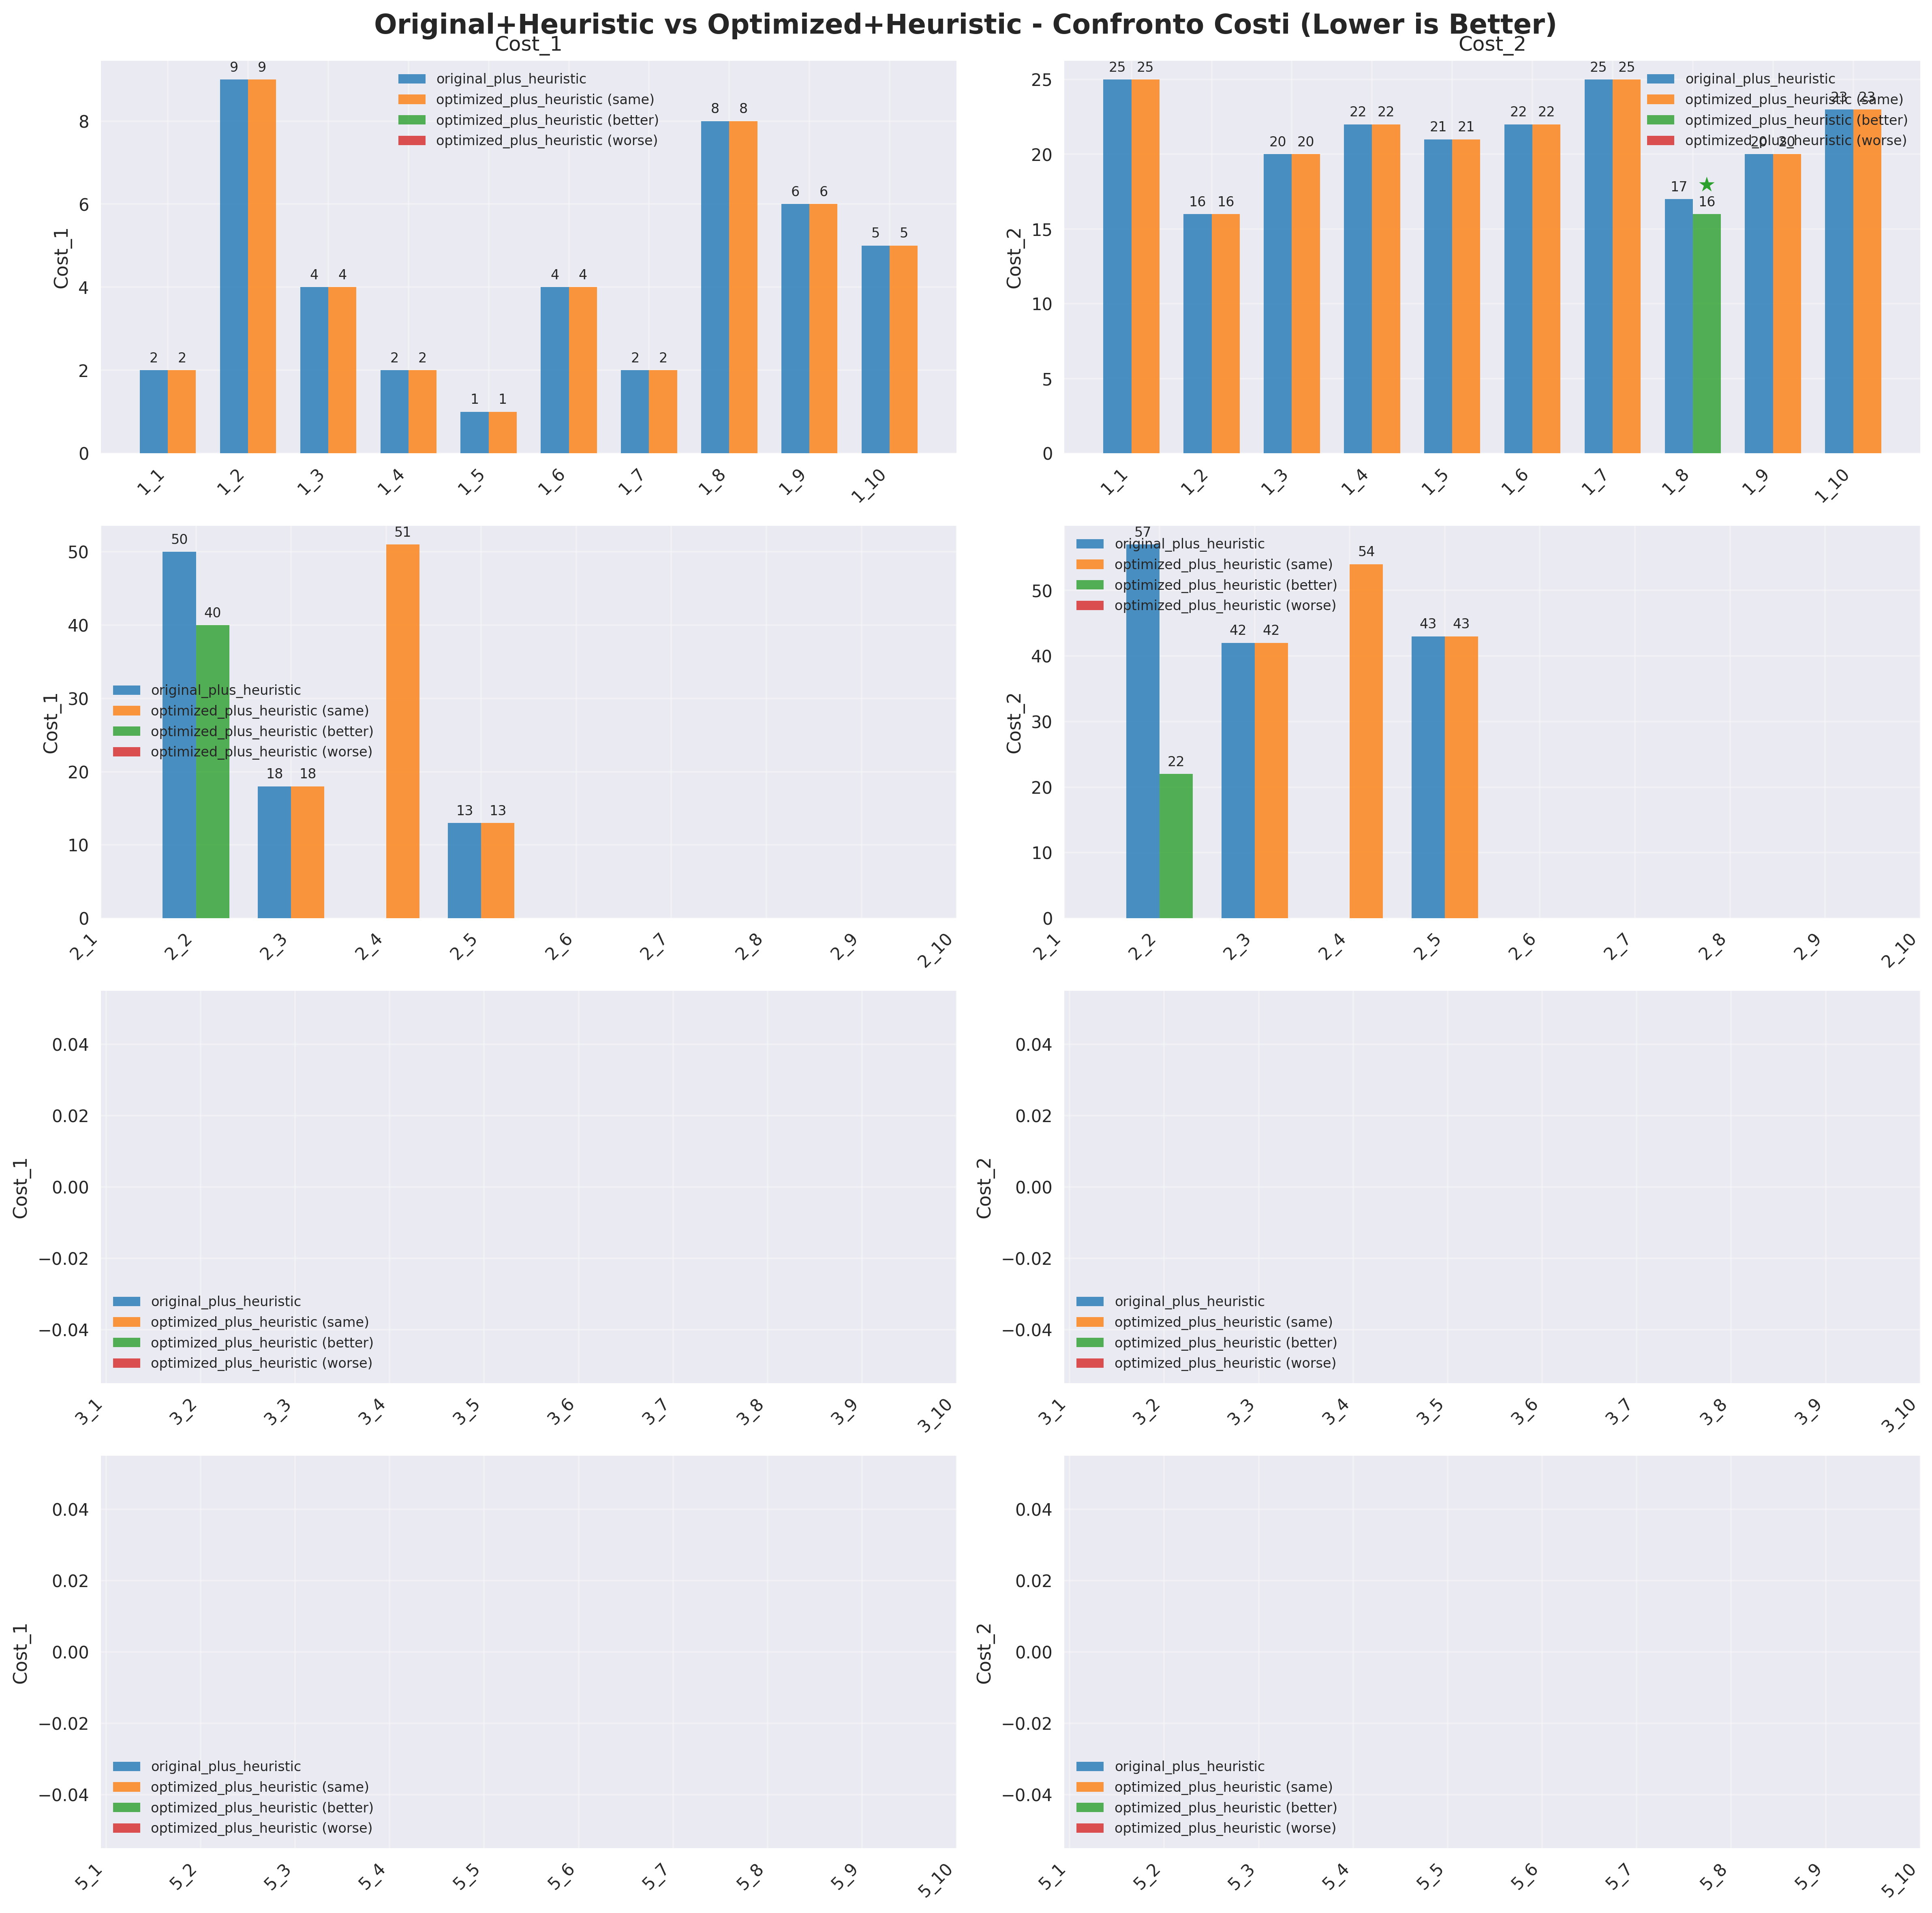
\includegraphics[width=0.9\textwidth]{../Results/graphs/cost_comparison_heuristic.png}
  \caption{Confronto dei costi tra codifica originale+euristica e ottimizzata+euristica. 
  Si osserva un leggero miglioramento su \texttt{cost\_2} per la versione ottimizzata.}
\end{figure}

\subsubsection{Optimized vs Optimized + Heuristic}
\begin{figure}[H]
  \centering
  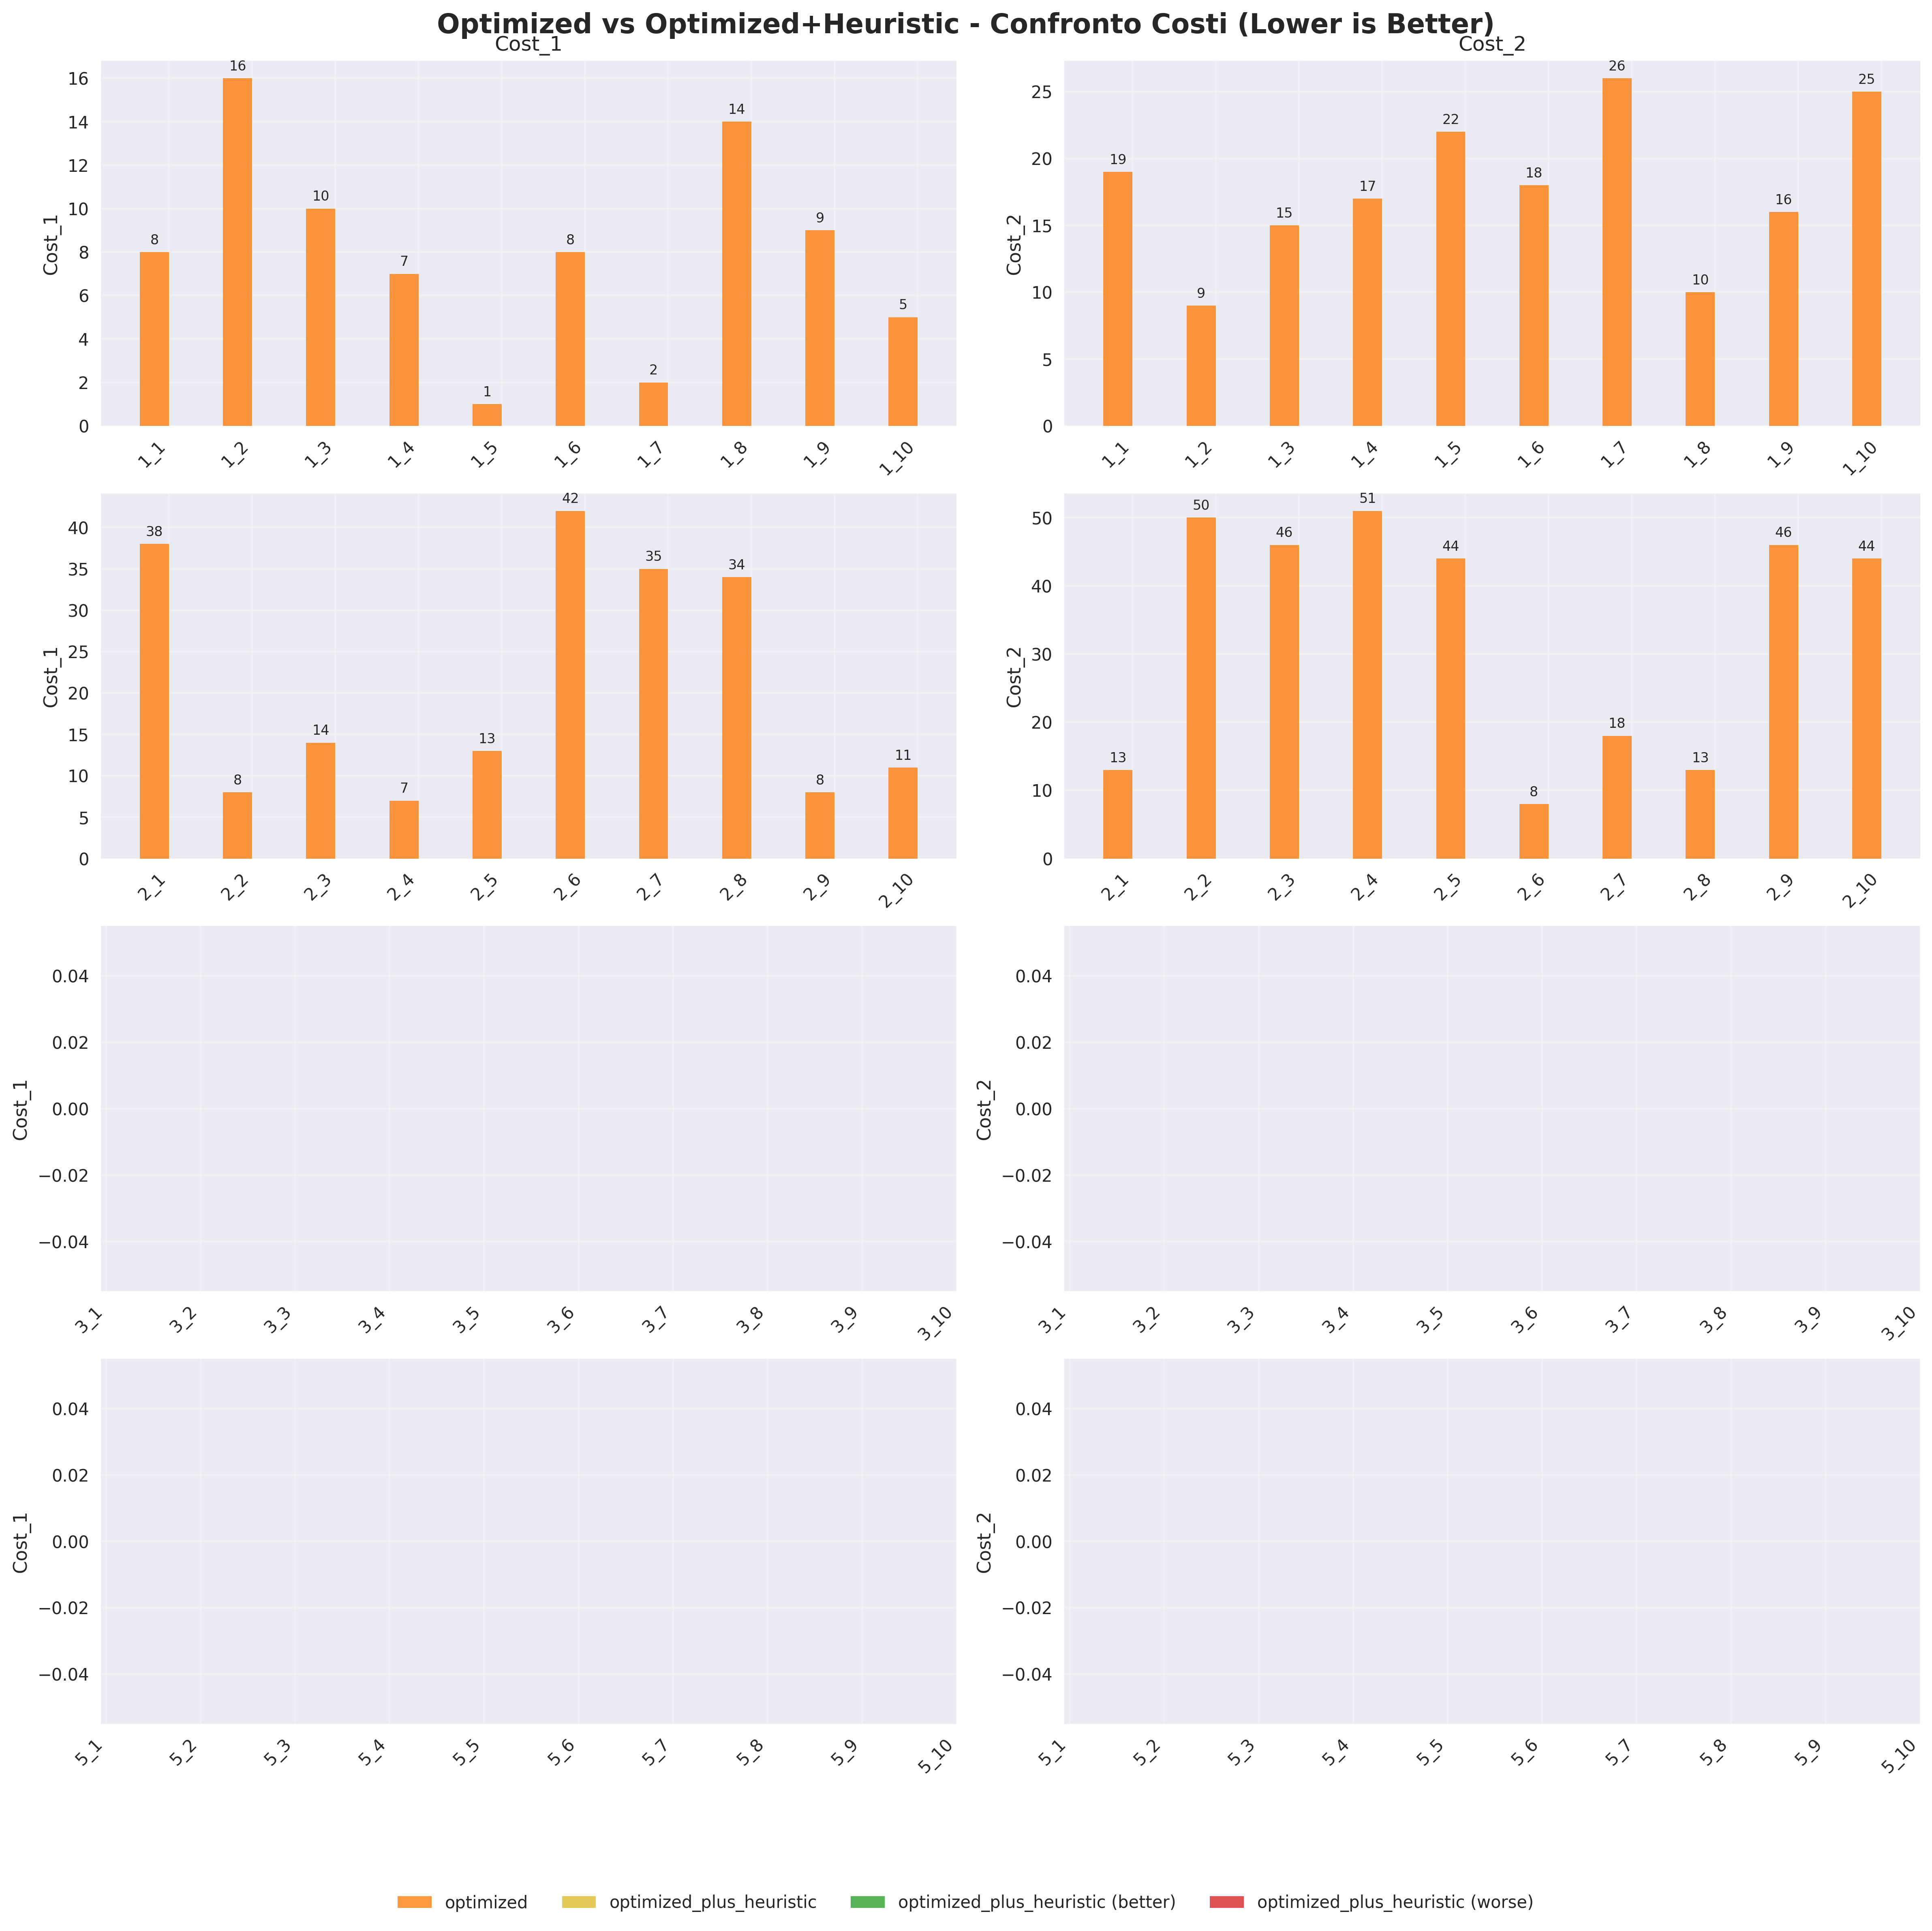
\includegraphics[width=0.9\textwidth]{../Results/graphs/cost_comparison_optimized_vs_optimized_heuristic.png}
  \caption{Confronto dei costi per configurazioni ottimizzate con e senza euristica. 
  L’aggiunta di euristiche non peggiora la qualità della soluzione.}
\end{figure}

\subsubsection{Original vs Optimized}
\begin{figure}[H]
  \centering
  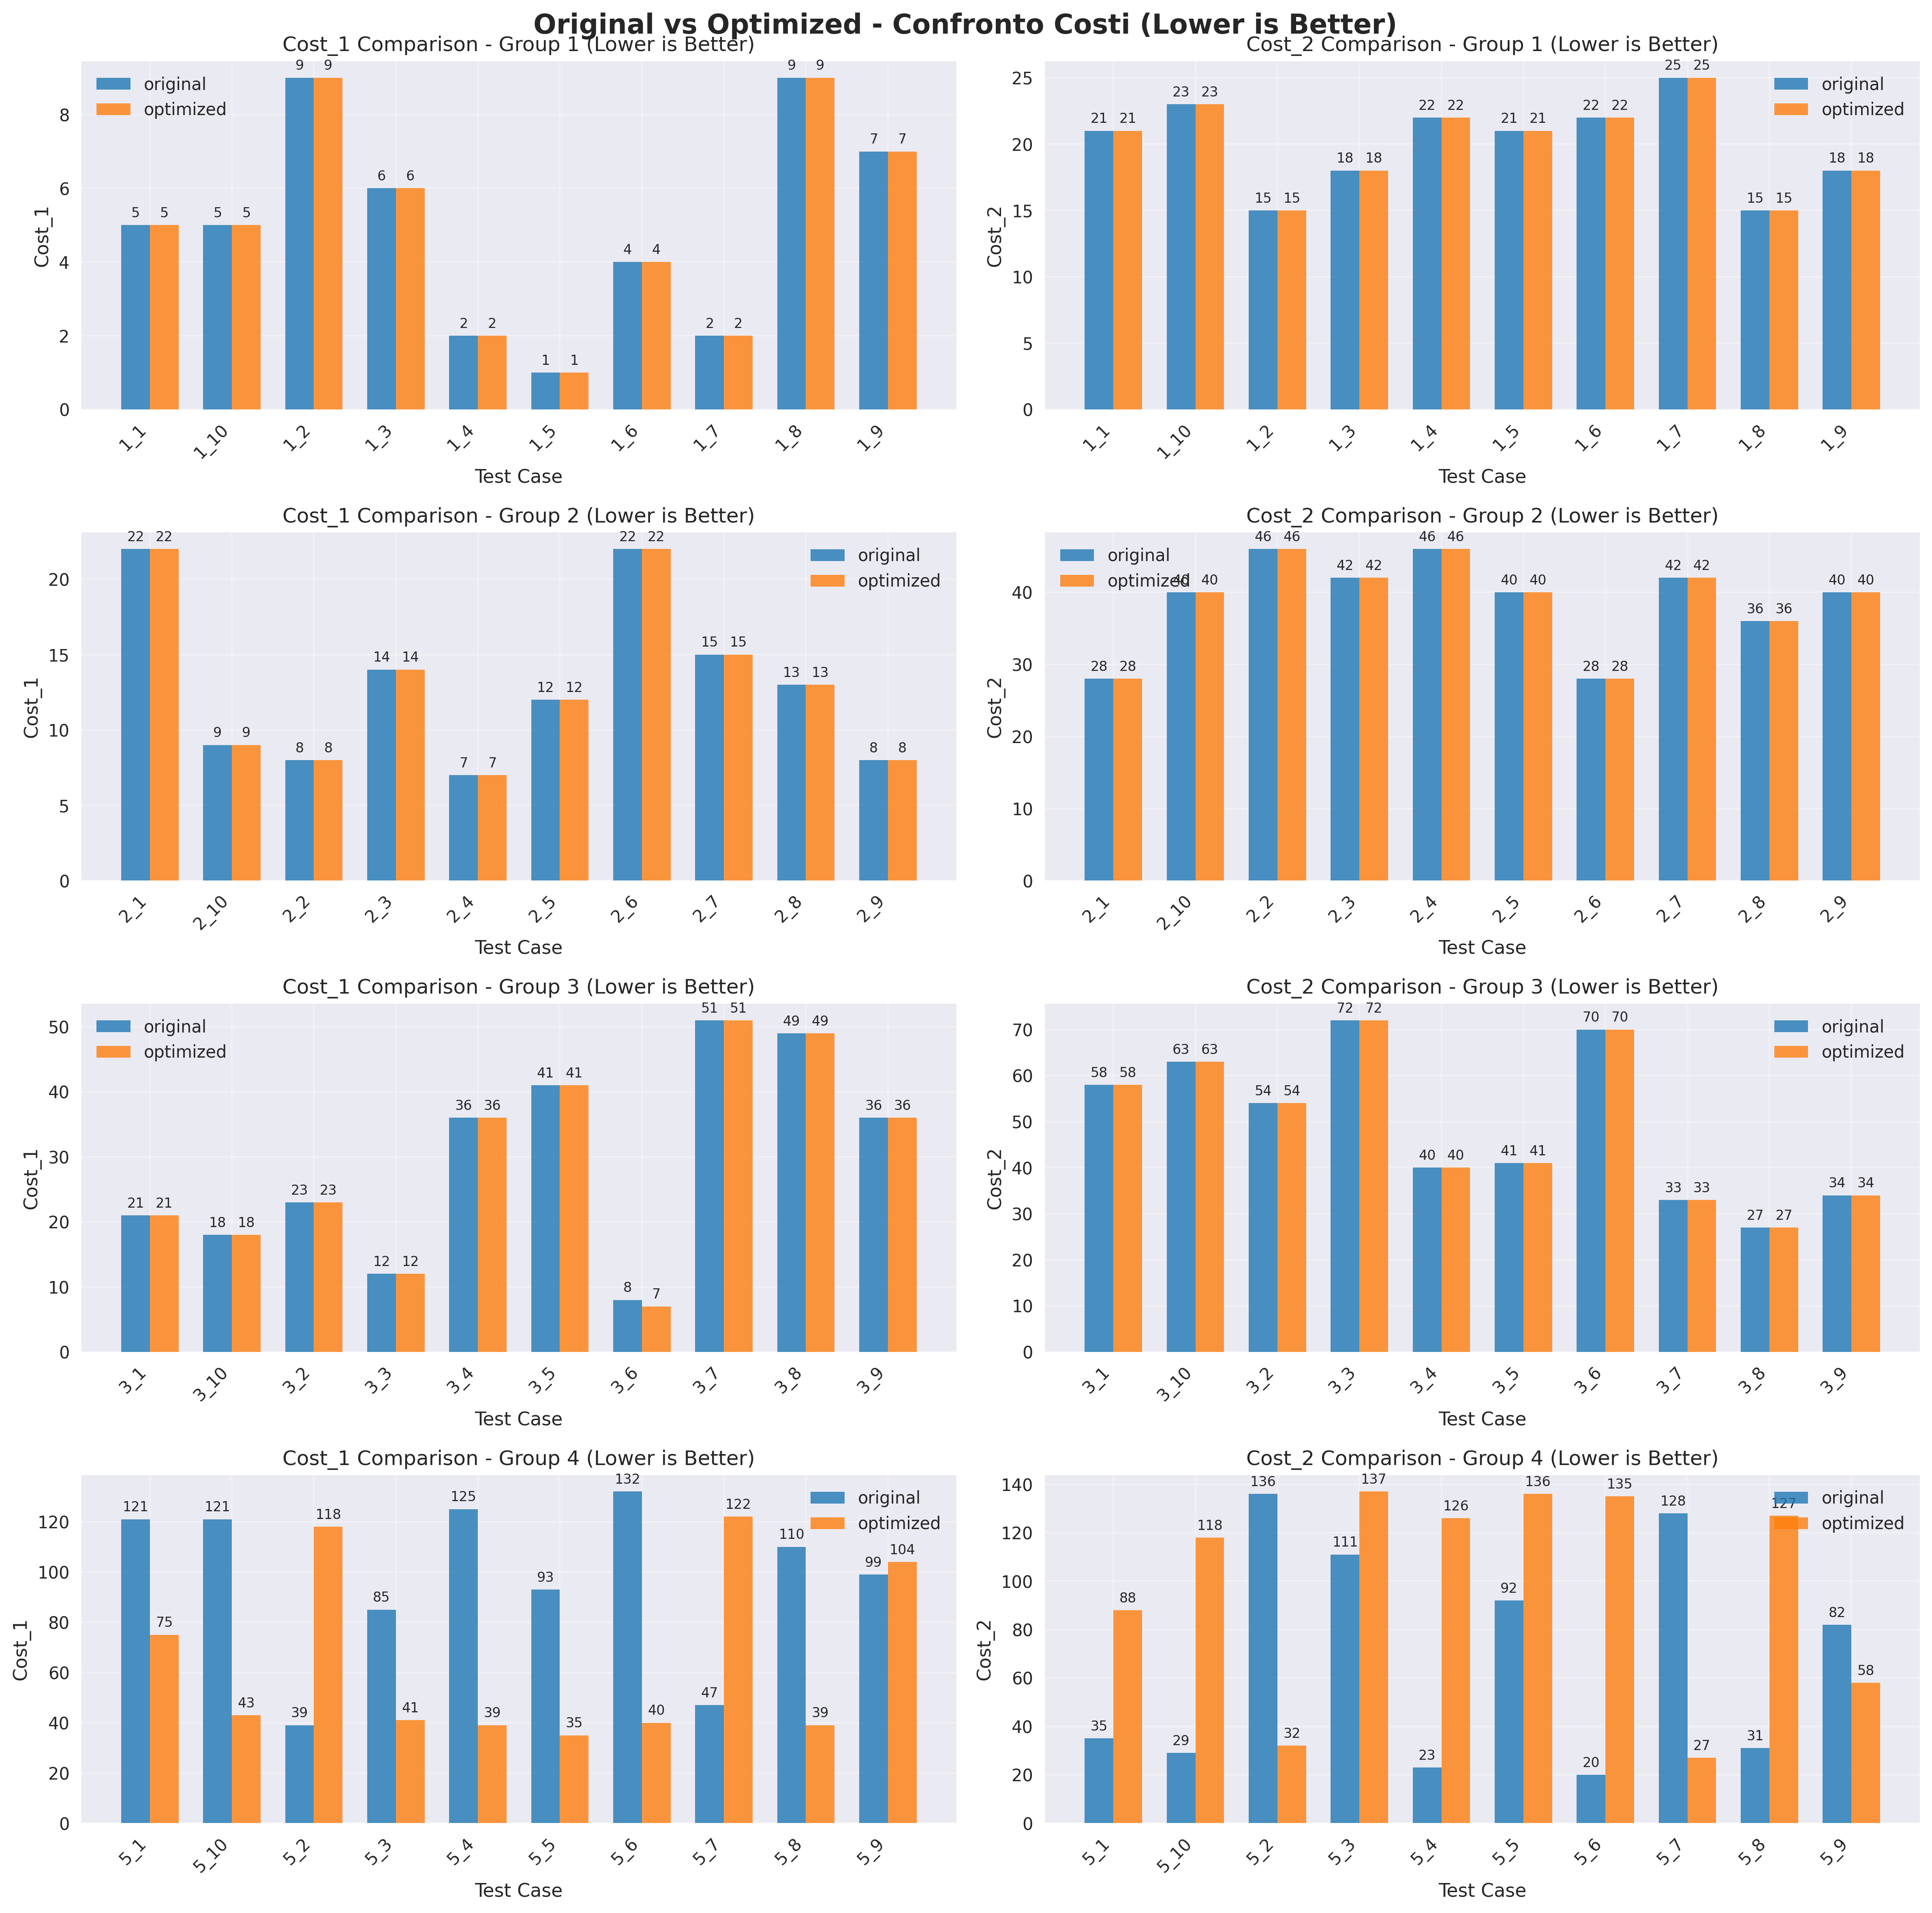
\includegraphics[width=0.9\textwidth]{../Results/graphs/cost_comparison_original_vs_optimized.png}
  \caption{Confronto dei costi tra codifica originale e ottimizzata. 
  L’ottimizzazione riduce marginalmente \texttt{cost\_1} su istanze complesse.}
\end{figure}

\subsubsection{Original vs Original + Heuristic}
\begin{figure}[H]
  \centering
  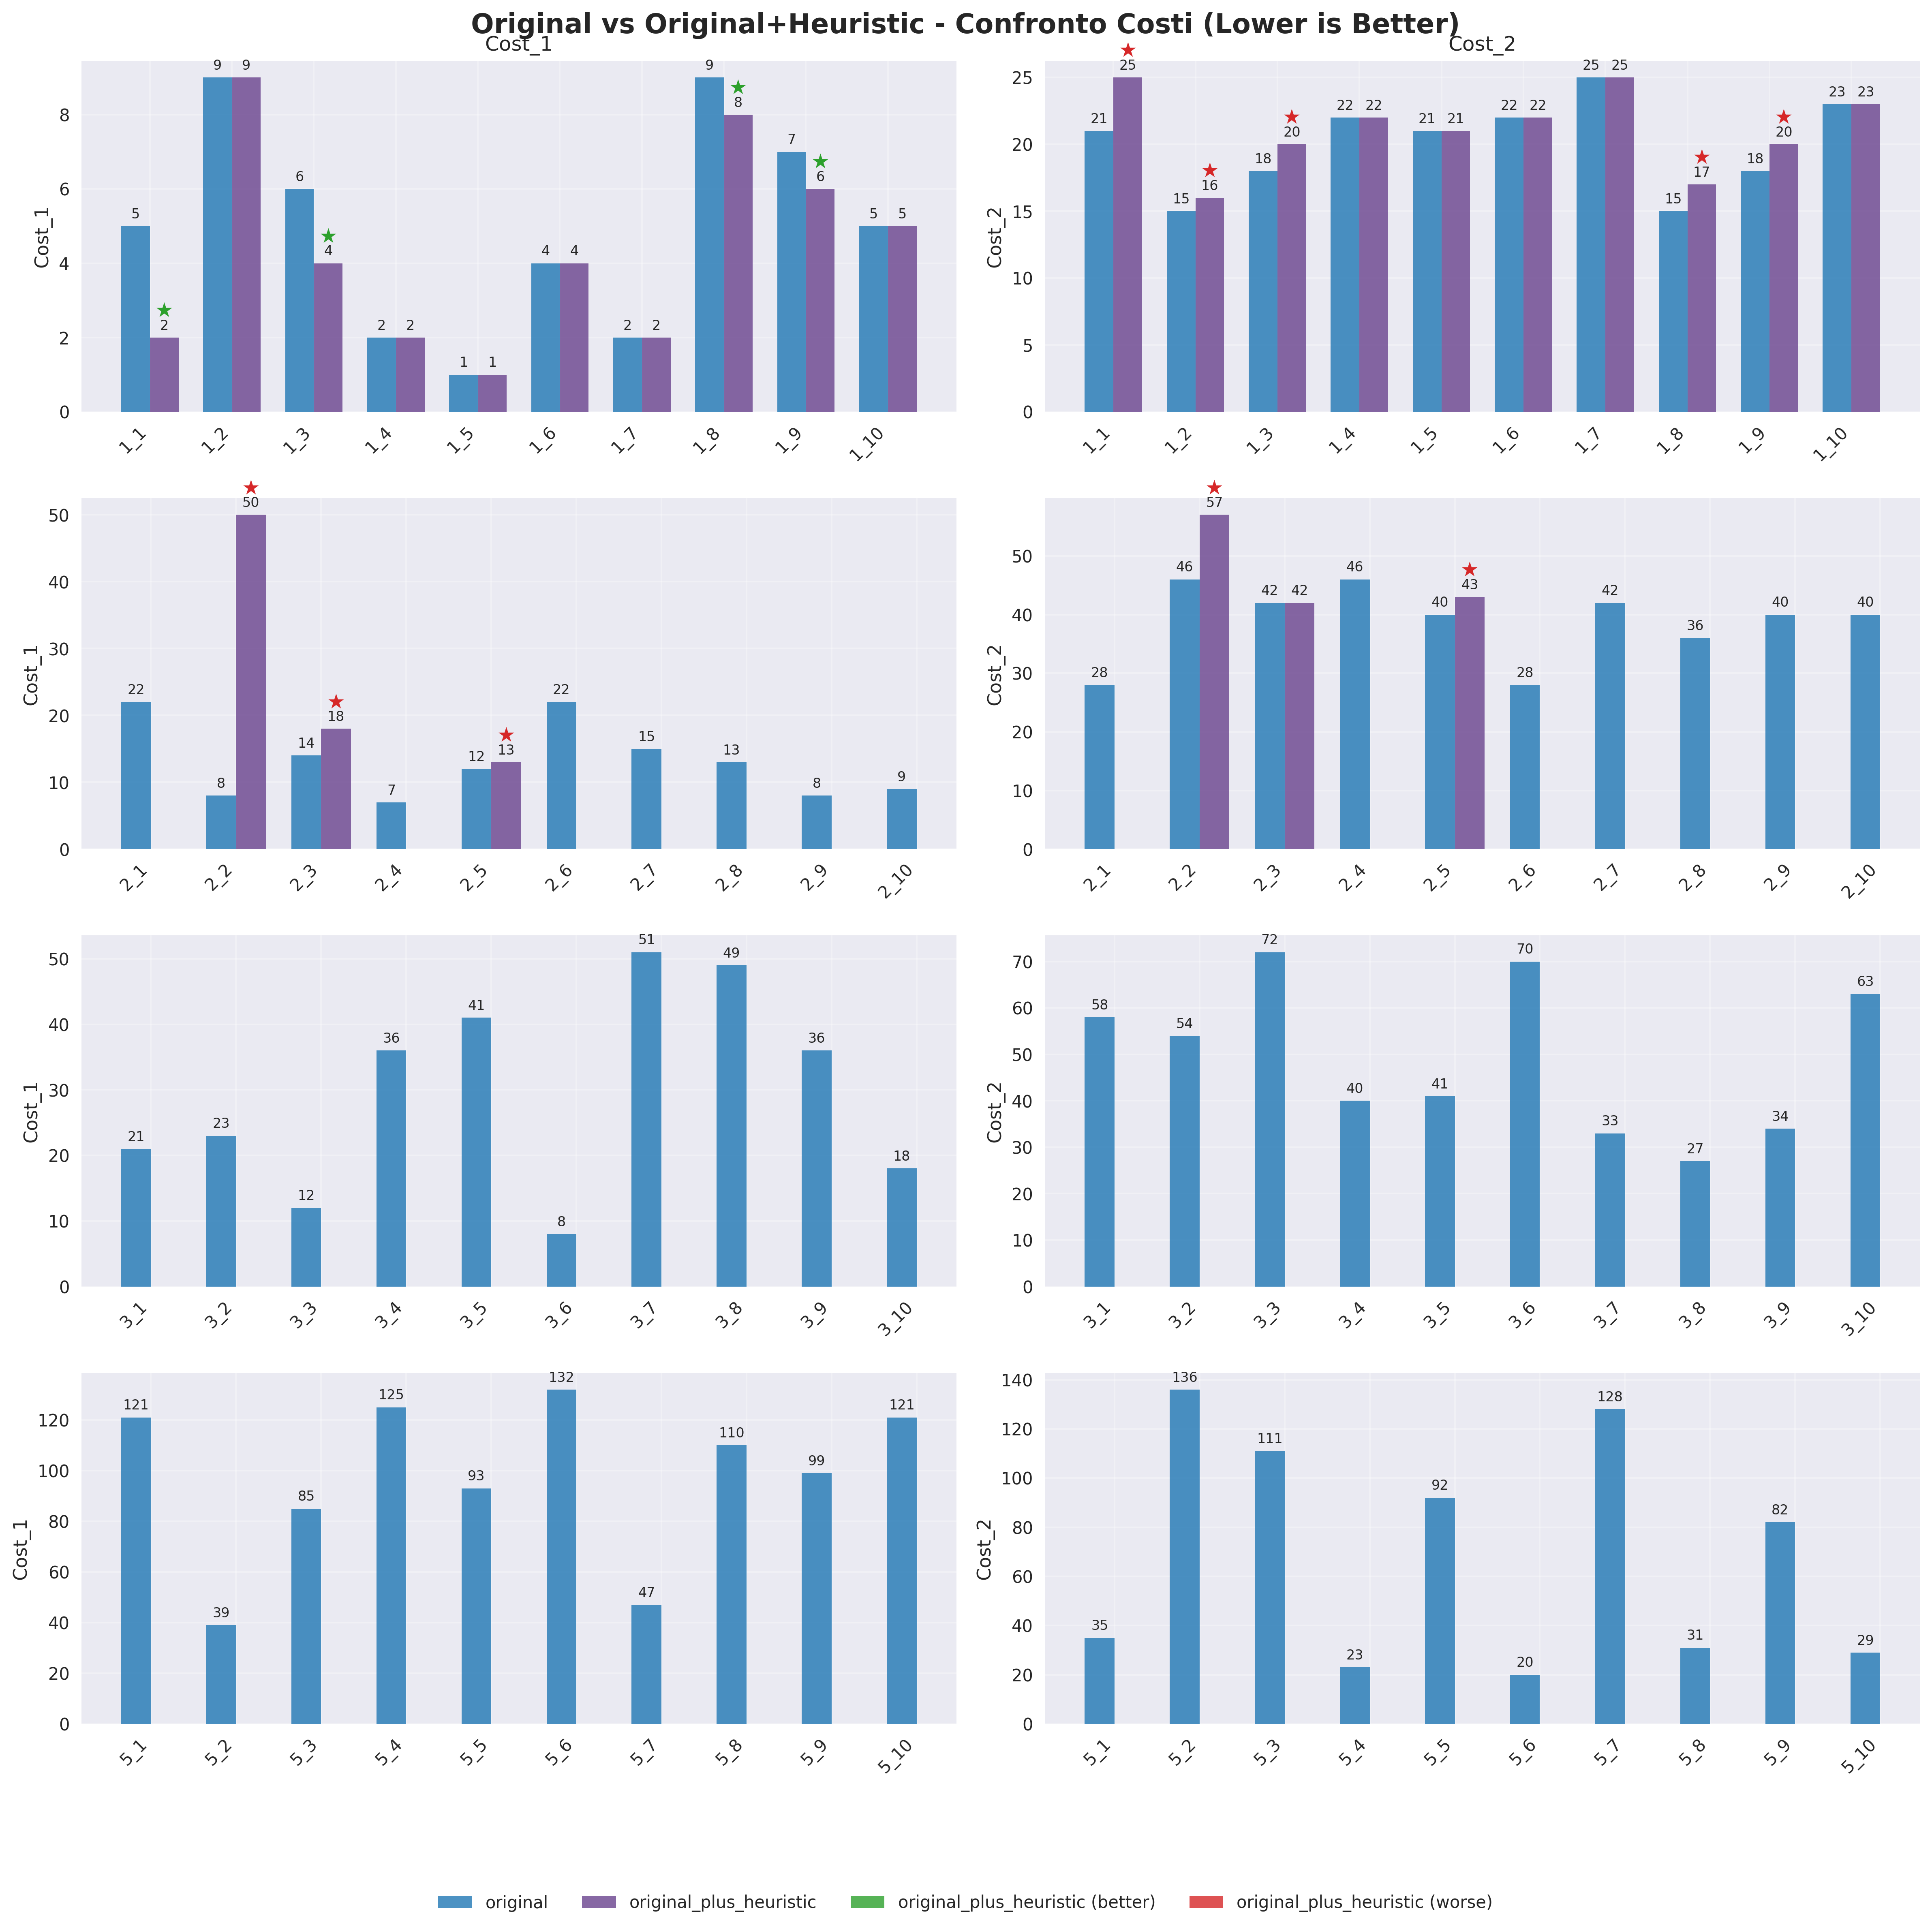
\includegraphics[width=0.9\textwidth]{../Results/graphs/cost_comparison_original_vs_original_heuristic.png}
  \caption{Confronto dei costi tra codifica originale e originale+euristica. 
  Euristiche singole non compromettono la qualità della soluzione.}
\end{figure}

\subsection{Confronto Tempi di Esecuzione}

\subsubsection{Original + Heuristic vs Optimized + Heuristic}
\begin{figure}[H]
  \centering
  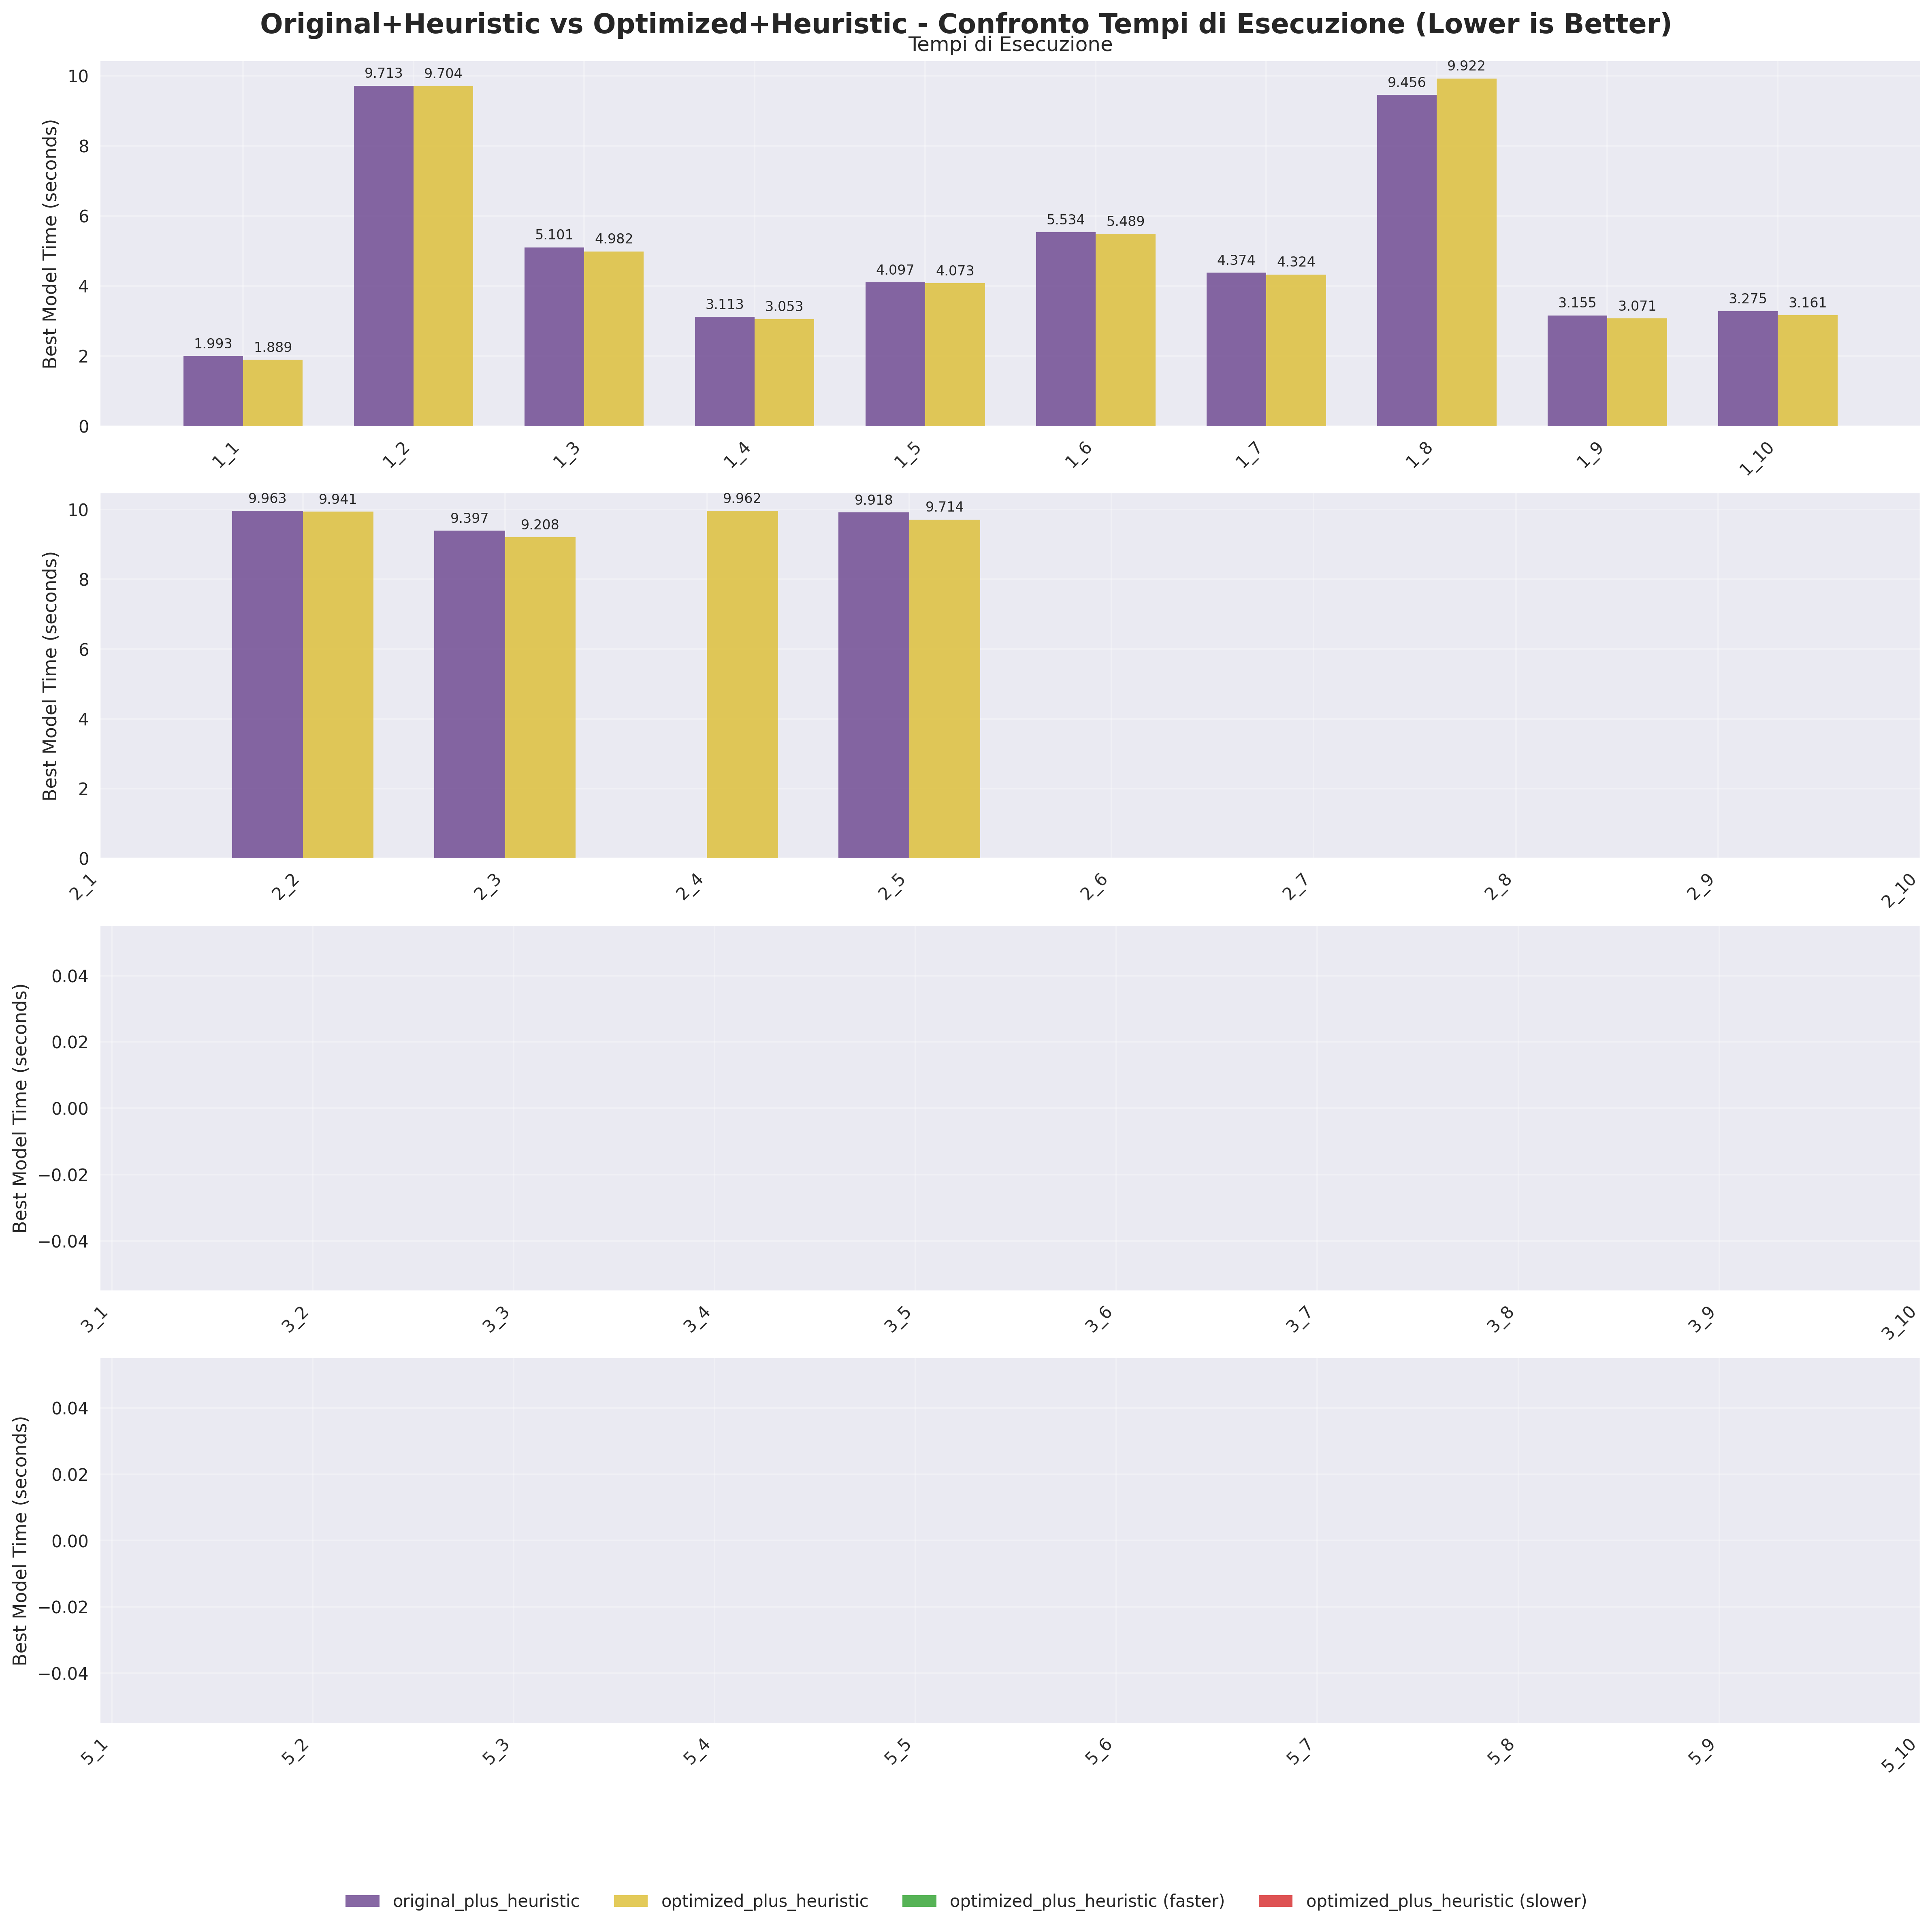
\includegraphics[width=0.9\textwidth]{../Results/graphs/time_comparison_heuristic.png}
  \caption{Tempi di esecuzione per versioni originale+euristica e ottimizzata+euristica. 
  Si nota un’accelerazione costante con la versione ottimizzata.}
\end{figure}

\subsubsection{Optimized vs Optimized + Heuristic}
\begin{figure}[H]
  \centering
  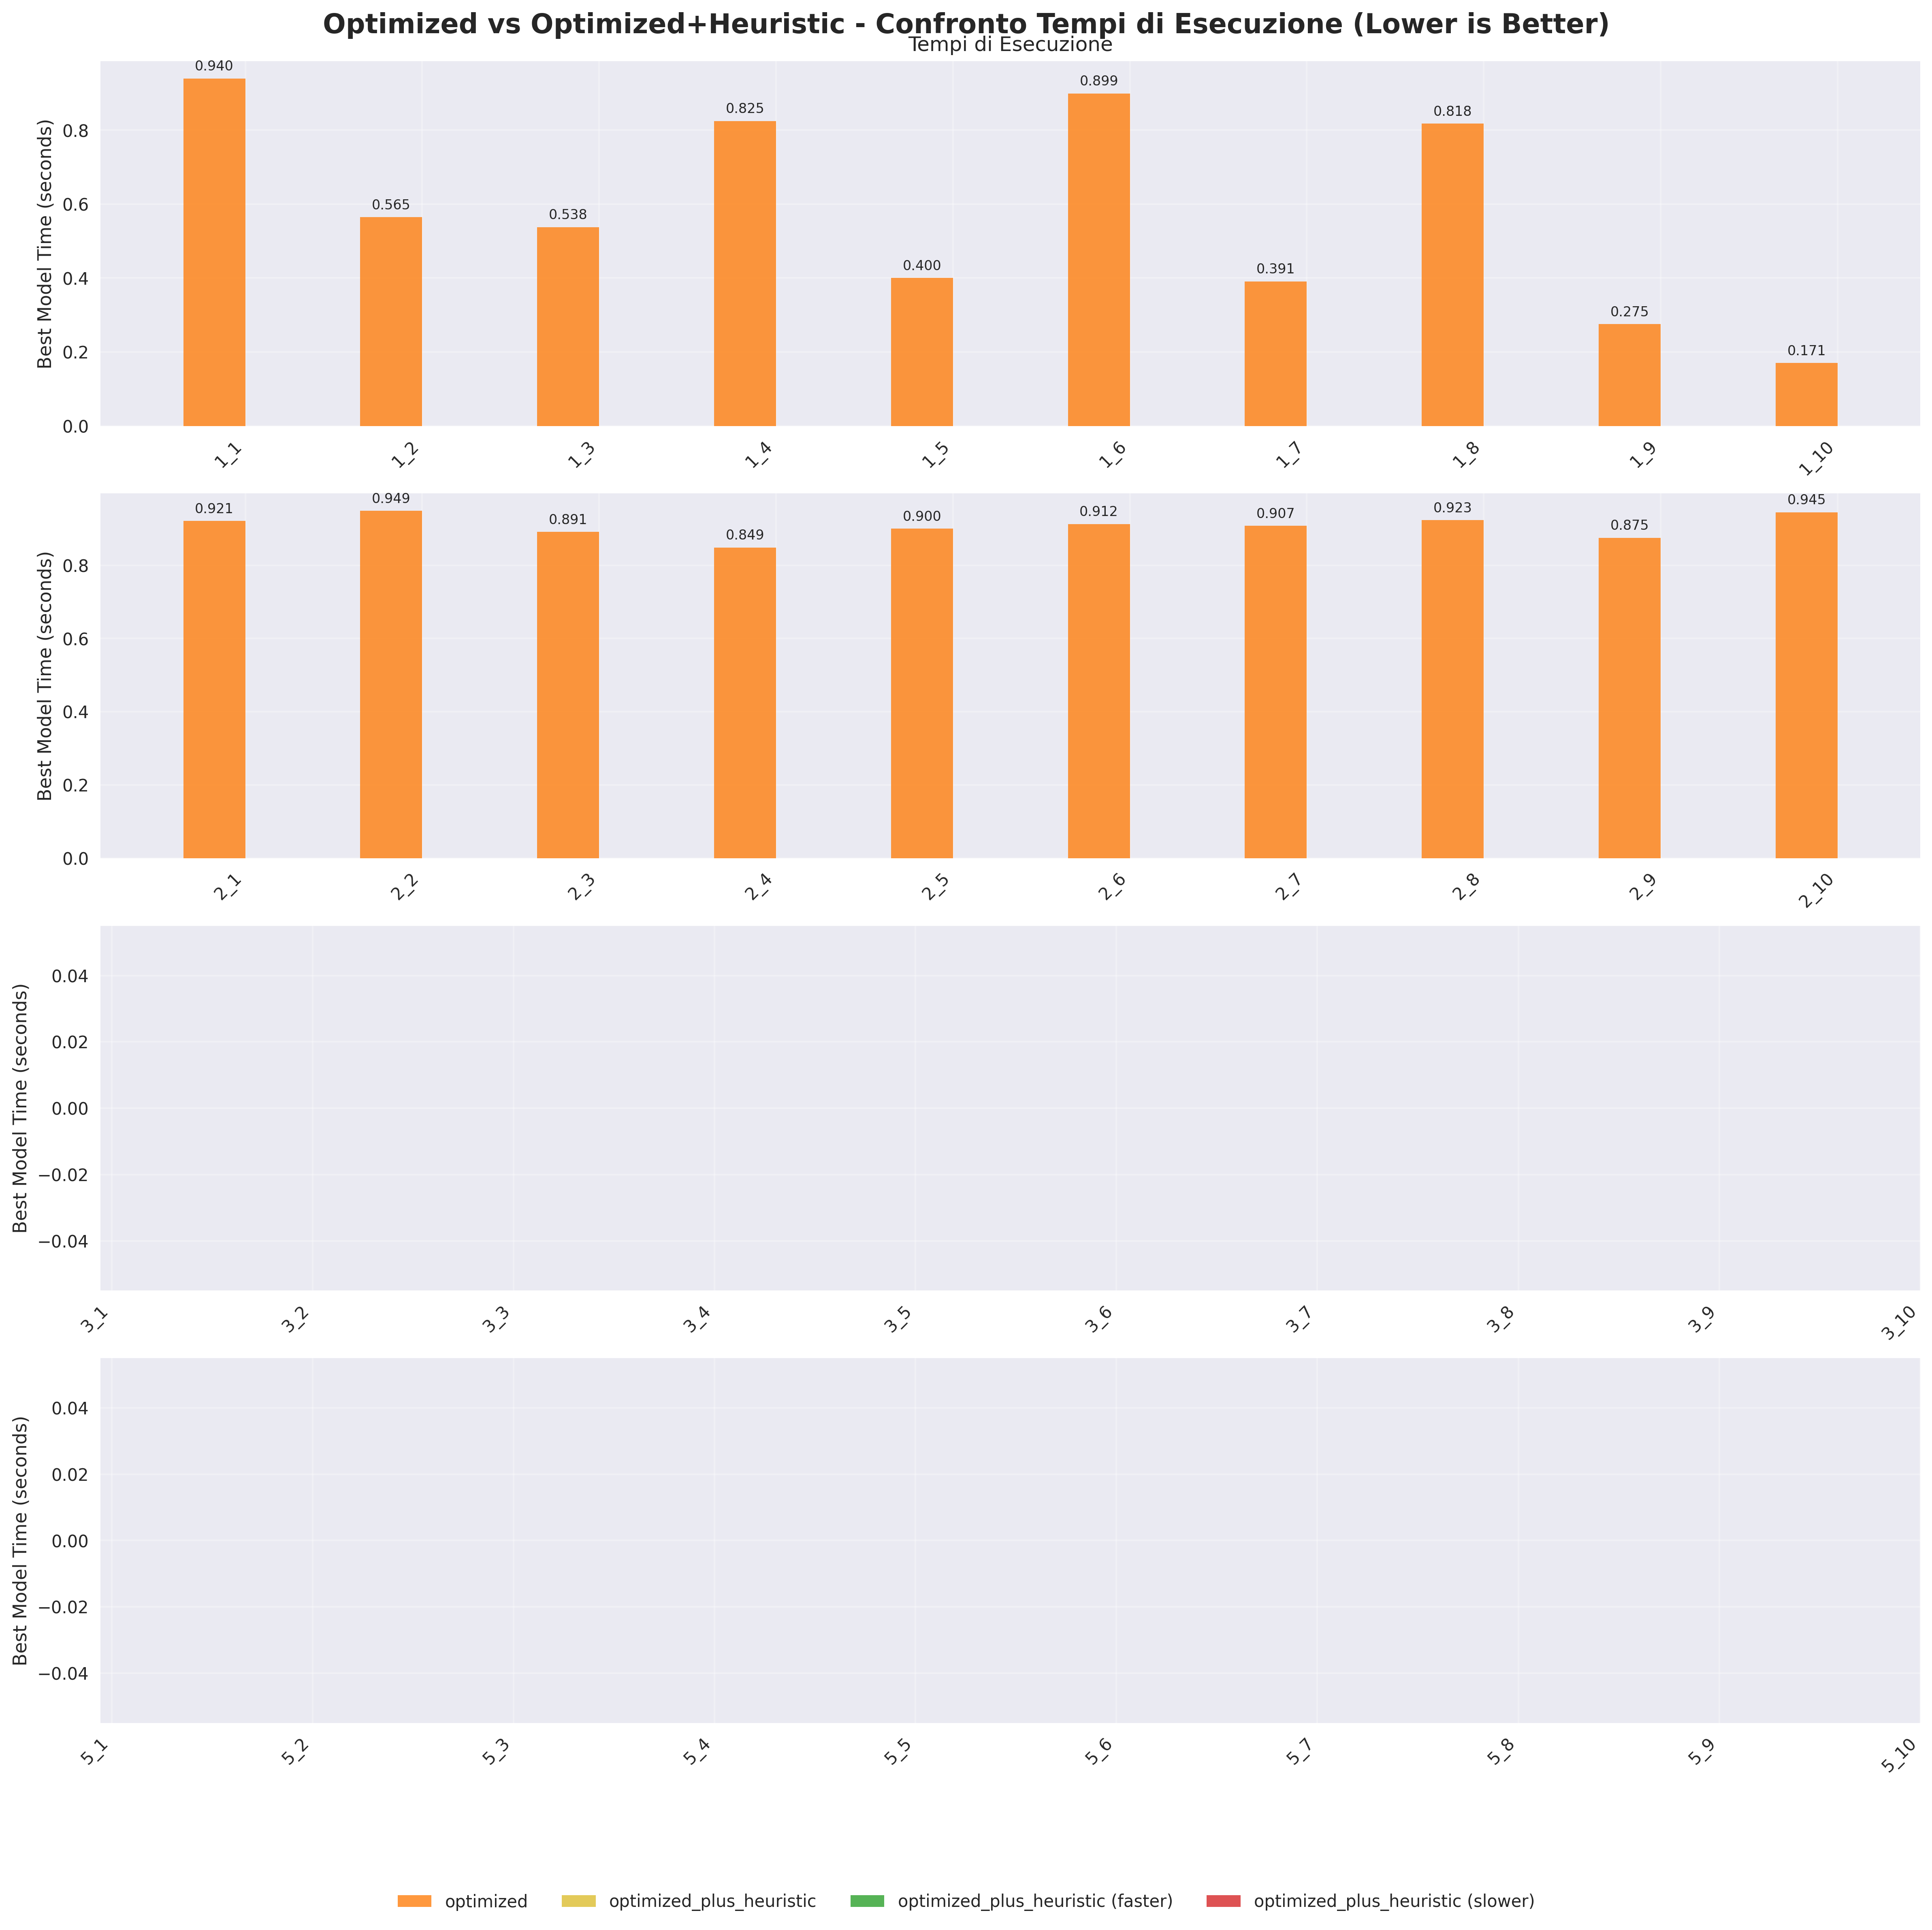
\includegraphics[width=0.9\textwidth]{../Results/graphs/time_comparison_optimized_vs_optimized_heuristic.png}
  \caption{Effetto delle euristiche sui tempi della versione ottimizzata. 
  Alcune istanze mostrano riduzioni fino a 6x nella discovery time.}
\end{figure}

\subsubsection{Original vs Optimized}
\begin{figure}[H]
  \centering
  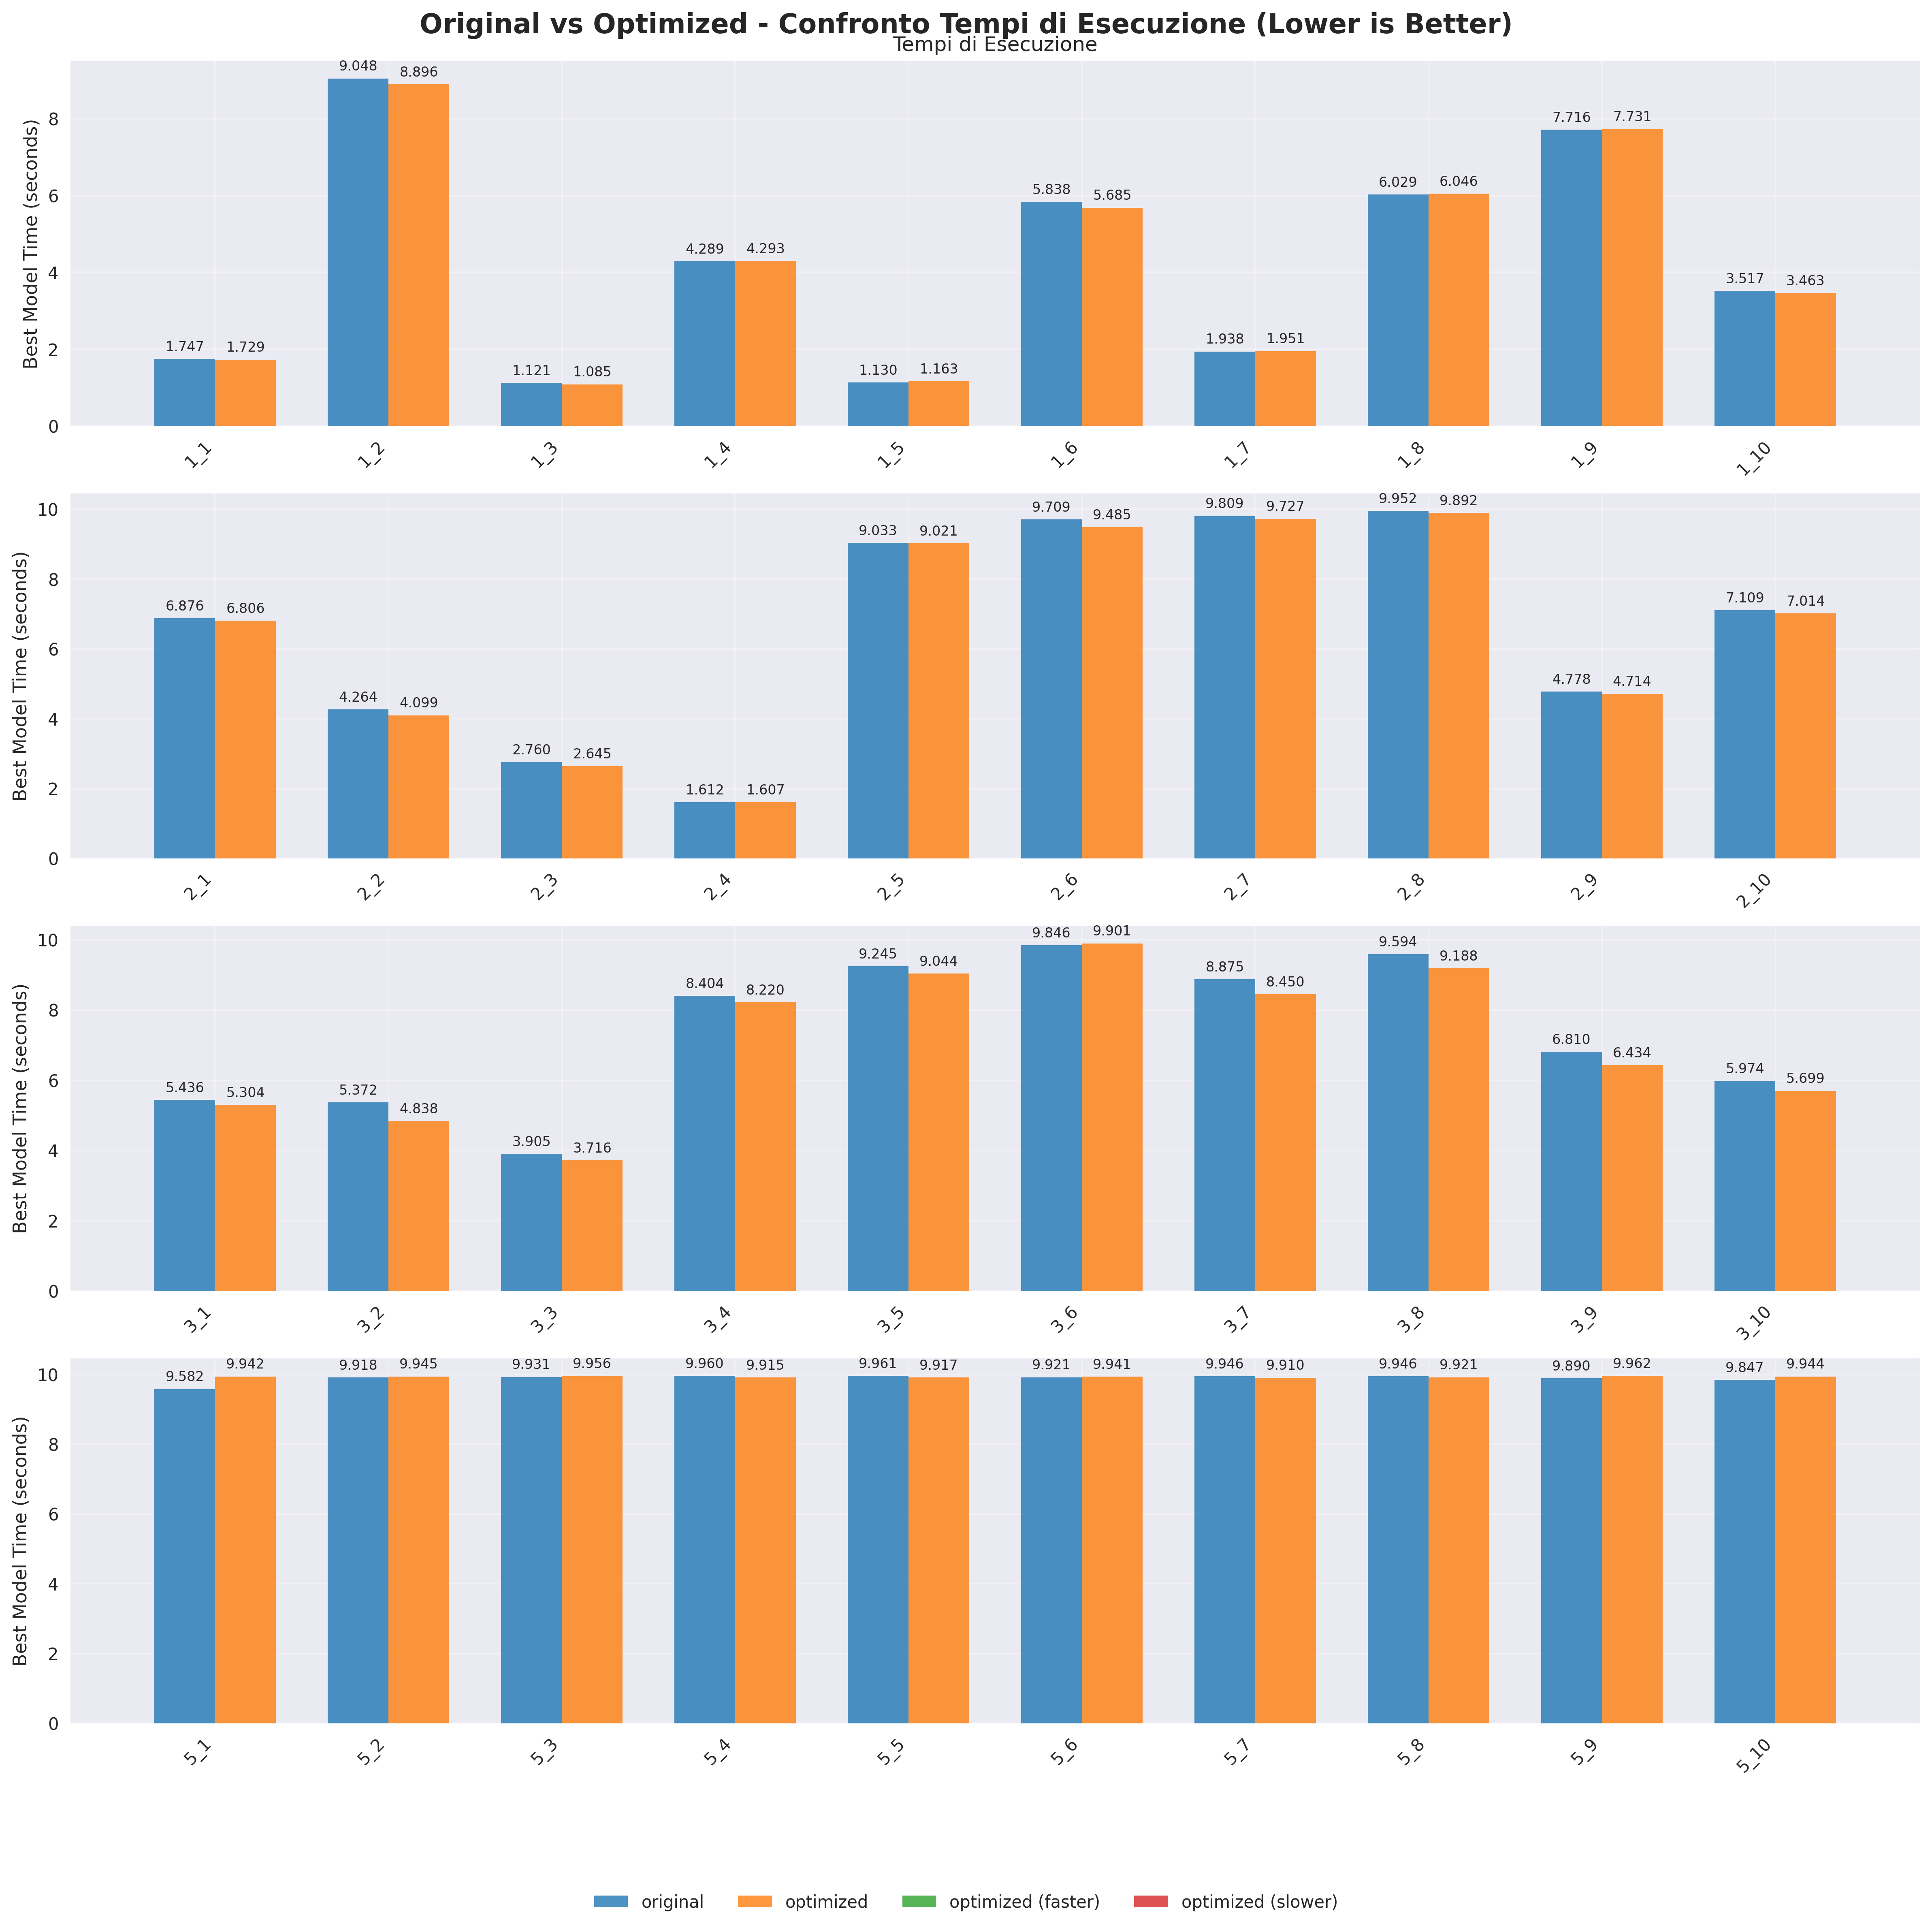
\includegraphics[width=0.9\textwidth]{../Results/graphs/time_comparison_original_vs_optimized.png}
  \caption{Confronto dei tempi tra codifica originale e ottimizzata. 
  L’ottimizzazione pura riduce significativamente i runtime sulle istanze medie.}
\end{figure}

\subsubsection{Original vs Original + Heuristic}
\begin{figure}[H]
  \centering
  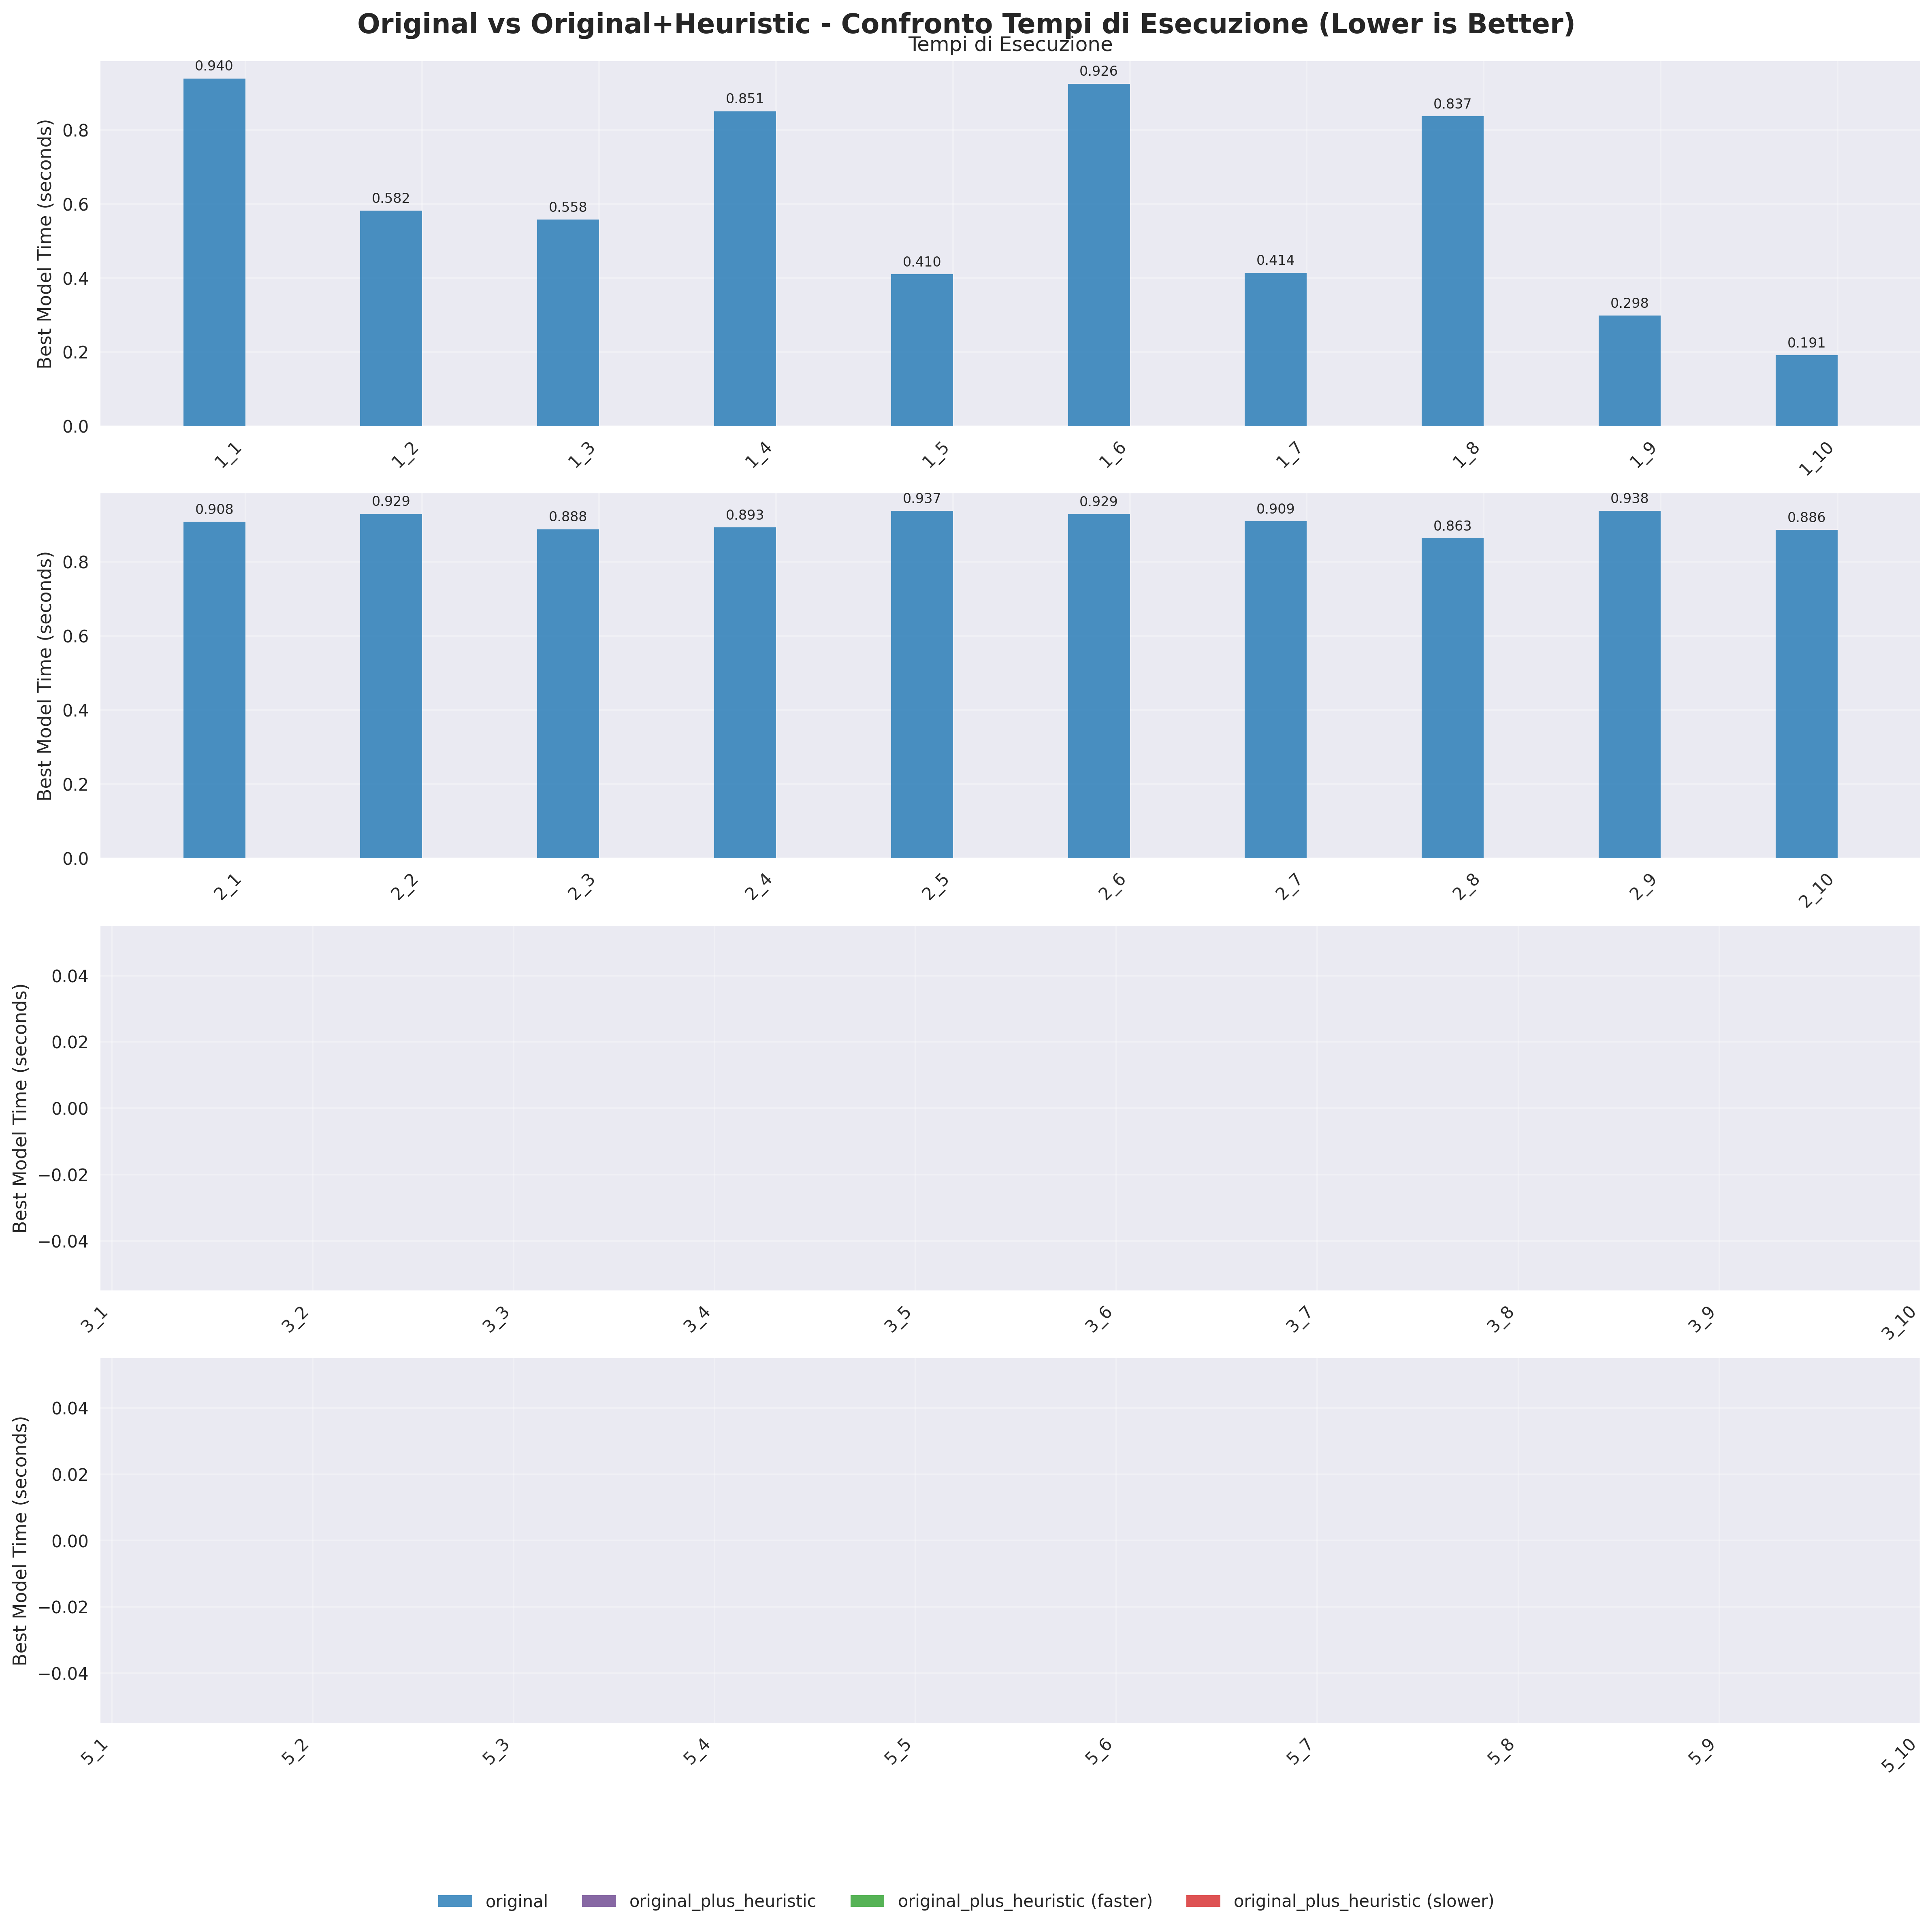
\includegraphics[width=0.9\textwidth]{../Results/graphs/time_comparison_original_vs_original_heuristic.png}
  \caption{Impatto delle euristiche sui tempi della codifica originale. 
  Euristiche isolate offrono variazioni moderate nei runtime.}
\end{figure}

\section{Conclusions and Future Research Directions}





\end{document}